\documentclass[twoside]{book}

% Packages required by doxygen
\usepackage{fixltx2e}
\usepackage{calc}
\usepackage{doxygen}
\usepackage[export]{adjustbox} % also loads graphicx
\usepackage{graphicx}
\usepackage[utf8]{inputenc}
\usepackage{makeidx}
\usepackage{multicol}
\usepackage{multirow}
\PassOptionsToPackage{warn}{textcomp}
\usepackage{textcomp}
\usepackage[nointegrals]{wasysym}
\usepackage[table]{xcolor}

% Font selection
\usepackage[T1]{fontenc}
\usepackage[scaled=.90]{helvet}
\usepackage{courier}
\usepackage{amssymb}
\usepackage{sectsty}
\renewcommand{\familydefault}{\sfdefault}
\allsectionsfont{%
  \fontseries{bc}\selectfont%
  \color{darkgray}%
}
\renewcommand{\DoxyLabelFont}{%
  \fontseries{bc}\selectfont%
  \color{darkgray}%
}
\newcommand{\+}{\discretionary{\mbox{\scriptsize$\hookleftarrow$}}{}{}}

% Page & text layout
\usepackage{geometry}
\geometry{%
  a4paper,%
  top=2.5cm,%
  bottom=2.5cm,%
  left=2.5cm,%
  right=2.5cm%
}
\tolerance=750
\hfuzz=15pt
\hbadness=750
\setlength{\emergencystretch}{15pt}
\setlength{\parindent}{0cm}
\setlength{\parskip}{3ex plus 2ex minus 2ex}
\makeatletter
\renewcommand{\paragraph}{%
  \@startsection{paragraph}{4}{0ex}{-1.0ex}{1.0ex}{%
    \normalfont\normalsize\bfseries\SS@parafont%
  }%
}
\renewcommand{\subparagraph}{%
  \@startsection{subparagraph}{5}{0ex}{-1.0ex}{1.0ex}{%
    \normalfont\normalsize\bfseries\SS@subparafont%
  }%
}
\makeatother

% Headers & footers
\usepackage{fancyhdr}
\pagestyle{fancyplain}
\fancyhead[LE]{\fancyplain{}{\bfseries\thepage}}
\fancyhead[CE]{\fancyplain{}{}}
\fancyhead[RE]{\fancyplain{}{\bfseries\leftmark}}
\fancyhead[LO]{\fancyplain{}{\bfseries\rightmark}}
\fancyhead[CO]{\fancyplain{}{}}
\fancyhead[RO]{\fancyplain{}{\bfseries\thepage}}
\fancyfoot[LE]{\fancyplain{}{}}
\fancyfoot[CE]{\fancyplain{}{}}
\fancyfoot[RE]{\fancyplain{}{\bfseries\scriptsize Generated by Doxygen }}
\fancyfoot[LO]{\fancyplain{}{\bfseries\scriptsize Generated by Doxygen }}
\fancyfoot[CO]{\fancyplain{}{}}
\fancyfoot[RO]{\fancyplain{}{}}
\renewcommand{\footrulewidth}{0.4pt}
\renewcommand{\chaptermark}[1]{%
  \markboth{#1}{}%
}
\renewcommand{\sectionmark}[1]{%
  \markright{\thesection\ #1}%
}

% Indices & bibliography
\usepackage{natbib}
\usepackage[titles]{tocloft}
\setcounter{tocdepth}{3}
\setcounter{secnumdepth}{5}
\makeindex

% Hyperlinks (required, but should be loaded last)
\usepackage{ifpdf}
\ifpdf
  \usepackage[pdftex,pagebackref=true]{hyperref}
\else
  \usepackage[ps2pdf,pagebackref=true]{hyperref}
\fi
\hypersetup{%
  colorlinks=true,%
  linkcolor=blue,%
  citecolor=blue,%
  unicode%
}

% Custom commands
\newcommand{\clearemptydoublepage}{%
  \newpage{\pagestyle{empty}\cleardoublepage}%
}

\usepackage{caption}
\captionsetup{labelsep=space,justification=centering,font={bf},singlelinecheck=off,skip=4pt,position=top}

%===== C O N T E N T S =====

\begin{document}

% Titlepage & ToC
\hypersetup{pageanchor=false,
             bookmarksnumbered=true,
             pdfencoding=unicode
            }
\pagenumbering{roman}
\begin{titlepage}
\vspace*{7cm}
\begin{center}%
{\Large My Project }\\
\vspace*{1cm}
{\large Generated by Doxygen 1.8.11}\\
\end{center}
\end{titlepage}
\clearemptydoublepage
\tableofcontents
\clearemptydoublepage
\pagenumbering{arabic}
\hypersetup{pageanchor=true}

%--- Begin generated contents ---
\chapter{Hierarchical Index}
\section{Class Hierarchy}
This inheritance list is sorted roughly, but not completely, alphabetically\+:\begin{DoxyCompactList}
\item \contentsline{section}{Element}{\pageref{classElement}}{}
\begin{DoxyCompactList}
\item \contentsline{section}{Ball}{\pageref{classBall}}{}
\item \contentsline{section}{Food\+Item}{\pageref{classFoodItem}}{}
\end{DoxyCompactList}
\item \contentsline{section}{Game\+Board}{\pageref{classGameBoard}}{}
\item \contentsline{section}{Player}{\pageref{classPlayer}}{}
\item \contentsline{section}{Stat}{\pageref{classStat}}{}
\item \contentsline{section}{Update\+Element\+Data}{\pageref{structUpdateElementData}}{}
\item \contentsline{section}{Web\+Server}{\pageref{classWebServer}}{}
\end{DoxyCompactList}

\chapter{Class Index}
\section{Class List}
Here are the classes, structs, unions and interfaces with brief descriptions\+:\begin{DoxyCompactList}
\item\contentsline{section}{\hyperlink{classBall}{Ball} }{\pageref{classBall}}{}
\item\contentsline{section}{\hyperlink{classElement}{Element} }{\pageref{classElement}}{}
\item\contentsline{section}{\hyperlink{classFoodItem}{Food\+Item} }{\pageref{classFoodItem}}{}
\item\contentsline{section}{\hyperlink{classGameBoard}{Game\+Board} }{\pageref{classGameBoard}}{}
\item\contentsline{section}{\hyperlink{classPlayer}{Player} }{\pageref{classPlayer}}{}
\item\contentsline{section}{\hyperlink{classStat}{Stat} }{\pageref{classStat}}{}
\item\contentsline{section}{\hyperlink{structUpdateElementData}{Update\+Element\+Data} }{\pageref{structUpdateElementData}}{}
\item\contentsline{section}{\hyperlink{classWebServer}{Web\+Server} }{\pageref{classWebServer}}{}
\end{DoxyCompactList}

\chapter{File Index}
\section{File List}
Here is a list of all documented files with brief descriptions\+:\begin{DoxyCompactList}
\item\contentsline{section}{{\bfseries ball.\+hpp} }{\pageref{ball_8hpp}}{}
\item\contentsline{section}{{\bfseries element.\+hpp} }{\pageref{element_8hpp}}{}
\item\contentsline{section}{{\bfseries food\+Item.\+hpp} }{\pageref{foodItem_8hpp}}{}
\item\contentsline{section}{{\bfseries game\+Board.\+hpp} }{\pageref{gameBoard_8hpp}}{}
\item\contentsline{section}{\hyperlink{main_8cpp}{main.\+cpp} }{\pageref{main_8cpp}}{}
\item\contentsline{section}{{\bfseries player.\+hpp} }{\pageref{player_8hpp}}{}
\item\contentsline{section}{{\bfseries stat.\+hpp} }{\pageref{stat_8hpp}}{}
\item\contentsline{section}{{\bfseries webserver.\+hpp} }{\pageref{webserver_8hpp}}{}
\end{DoxyCompactList}

\chapter{Class Documentation}
\hypertarget{classBall}{}\section{Ball Class Reference}
\label{classBall}\index{Ball@{Ball}}


Inheritance diagram for Ball\+:
\nopagebreak
\begin{figure}[H]
\begin{center}
\leavevmode
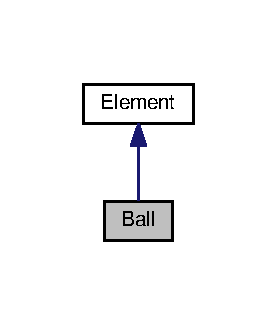
\includegraphics[width=133pt]{classBall__inherit__graph}
\end{center}
\end{figure}


Collaboration diagram for Ball\+:
\nopagebreak
\begin{figure}[H]
\begin{center}
\leavevmode
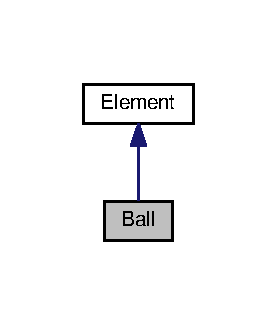
\includegraphics[width=133pt]{classBall__coll__graph}
\end{center}
\end{figure}
\subsection*{Public Member Functions}
\begin{DoxyCompactItemize}
\item 
virtual void {\bfseries notify} ()\hypertarget{classBall_aac709d26ebeb71a87af845dc8c2316a2}{}\label{classBall_aac709d26ebeb71a87af845dc8c2316a2}

\item 
void {\bfseries increase\+Mass} (int add\+\_\+mass)\hypertarget{classBall_a39e9307ae41f0b651315c5d0dbb30b73}{}\label{classBall_a39e9307ae41f0b651315c5d0dbb30b73}

\end{DoxyCompactItemize}


The documentation for this class was generated from the following file\+:\begin{DoxyCompactItemize}
\item 
ball.\+hpp\end{DoxyCompactItemize}

\hypertarget{classElement}{}\section{Element Class Reference}
\label{classElement}\index{Element@{Element}}


Inheritance diagram for Element\+:
\nopagebreak
\begin{figure}[H]
\begin{center}
\leavevmode
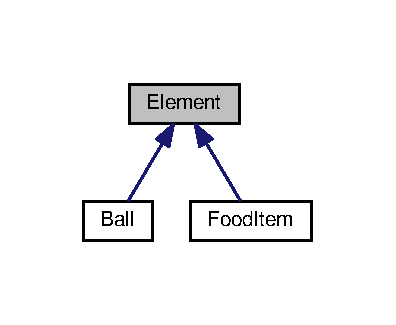
\includegraphics[width=190pt]{classElement__inherit__graph}
\end{center}
\end{figure}
\subsection*{Public Member Functions}
\begin{DoxyCompactItemize}
\item 
virtual void {\bfseries notify} ()=0\hypertarget{classElement_a3374a4e8de32e7f1c80d63deaec4d1b2}{}\label{classElement_a3374a4e8de32e7f1c80d63deaec4d1b2}

\end{DoxyCompactItemize}


The documentation for this class was generated from the following files\+:\begin{DoxyCompactItemize}
\item 
element.\+hpp\item 
element.\+cpp\end{DoxyCompactItemize}

\hypertarget{classFoodItem}{}\section{Food\+Item Class Reference}
\label{classFoodItem}\index{Food\+Item@{Food\+Item}}


Inheritance diagram for Food\+Item\+:
\nopagebreak
\begin{figure}[H]
\begin{center}
\leavevmode
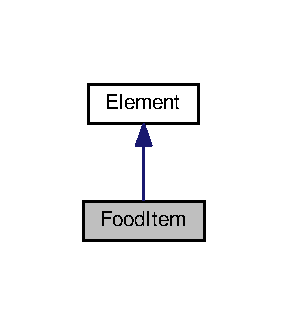
\includegraphics[width=138pt]{classFoodItem__inherit__graph}
\end{center}
\end{figure}


Collaboration diagram for Food\+Item\+:
\nopagebreak
\begin{figure}[H]
\begin{center}
\leavevmode
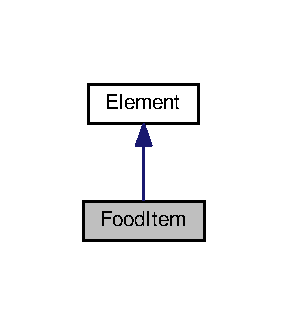
\includegraphics[width=138pt]{classFoodItem__coll__graph}
\end{center}
\end{figure}
\subsection*{Public Member Functions}
\begin{DoxyCompactItemize}
\item 
virtual void {\bfseries notify} ()\hypertarget{classFoodItem_ad7c00abb43b23475db4e60c87f98eb86}{}\label{classFoodItem_ad7c00abb43b23475db4e60c87f98eb86}

\end{DoxyCompactItemize}


The documentation for this class was generated from the following file\+:\begin{DoxyCompactItemize}
\item 
food\+Item.\+hpp\end{DoxyCompactItemize}

\hypertarget{classGameBoard}{}\section{Game\+Board Class Reference}
\label{classGameBoard}\index{Game\+Board@{Game\+Board}}
\subsection*{Public Member Functions}
\begin{DoxyCompactItemize}
\item 
void {\bfseries run} ()\hypertarget{classGameBoard_a9333dcacc4d45c25b0ee45ba0e48ac05}{}\label{classGameBoard_a9333dcacc4d45c25b0ee45ba0e48ac05}

\item 
void {\bfseries detect\+Collision} ()\hypertarget{classGameBoard_ae7f5e99ff3dfdaa9e7270fd4ac15fc61}{}\label{classGameBoard_ae7f5e99ff3dfdaa9e7270fd4ac15fc61}

\item 
void {\bfseries add\+New\+Player} ()\hypertarget{classGameBoard_ab6d586c018f78ef4128fb495bc4b6051}{}\label{classGameBoard_ab6d586c018f78ef4128fb495bc4b6051}

\item 
void {\bfseries delete\+Player} ()\hypertarget{classGameBoard_a3d710da0c96e2c1ffb9e63d8b896d16b}{}\label{classGameBoard_a3d710da0c96e2c1ffb9e63d8b896d16b}

\item 
void {\bfseries add\+New\+Food} ()\hypertarget{classGameBoard_ae2d6446a9ec3508e2259184d75da035c}{}\label{classGameBoard_ae2d6446a9ec3508e2259184d75da035c}

\item 
void {\bfseries delete\+Food} ()\hypertarget{classGameBoard_a5bdf02b93303dcf7a1415ee4a340cd48}{}\label{classGameBoard_a5bdf02b93303dcf7a1415ee4a340cd48}

\item 
void {\bfseries create\+Initial\+Food} ()\hypertarget{classGameBoard_a193c7dce603f0e6fde5d497a8fe5509a}{}\label{classGameBoard_a193c7dce603f0e6fde5d497a8fe5509a}

\item 
void {\bfseries update} ()\hypertarget{classGameBoard_a5dc2bdedeaa9d70bb4a1c35a5a257d91}{}\label{classGameBoard_a5dc2bdedeaa9d70bb4a1c35a5a257d91}

\end{DoxyCompactItemize}
\subsection*{Static Public Member Functions}
\begin{DoxyCompactItemize}
\item 
static void {\bfseries get\+Instance} ()\hypertarget{classGameBoard_a7ac1ba55db2c8d0fa666ac73ea3d2adb}{}\label{classGameBoard_a7ac1ba55db2c8d0fa666ac73ea3d2adb}

\end{DoxyCompactItemize}


The documentation for this class was generated from the following files\+:\begin{DoxyCompactItemize}
\item 
game\+Board.\+hpp\item 
game\+Board.\+cpp\end{DoxyCompactItemize}

\hypertarget{classPlayer}{}\section{Player Class Reference}
\label{classPlayer}\index{Player@{Player}}
\subsection*{Public Member Functions}
\begin{DoxyCompactItemize}
\item 
\hyperlink{classPlayer_ab5c49386411a5e649c8a6328d5a510f8}{constructor} (id, x, y, r, color, name)
\begin{DoxyCompactList}\small\item\em \hyperlink{classPlayer}{Player} constructor. \end{DoxyCompactList}\item 
\hyperlink{classPlayer_a619a6d875382df23fcd0cf423e233b3a}{show} ()
\begin{DoxyCompactList}\small\item\em Display player on screen. \end{DoxyCompactList}\end{DoxyCompactItemize}


\subsection{Member Function Documentation}
\index{Player@{Player}!constructor@{constructor}}
\index{constructor@{constructor}!Player@{Player}}
\subsubsection[{\texorpdfstring{constructor(id, x, y, r, color, name)}{constructor(id, x, y, r, color, name)}}]{\setlength{\rightskip}{0pt plus 5cm}Player\+::constructor (
\begin{DoxyParamCaption}
\item[{}]{id, }
\item[{}]{x, }
\item[{}]{y, }
\item[{}]{r, }
\item[{}]{color, }
\item[{}]{name}
\end{DoxyParamCaption}
)\hspace{0.3cm}{\ttfamily [inline]}}\hypertarget{classPlayer_ab5c49386411a5e649c8a6328d5a510f8}{}\label{classPlayer_ab5c49386411a5e649c8a6328d5a510f8}


\hyperlink{classPlayer}{Player} constructor. 

\index{Player@{Player}!show@{show}}
\index{show@{show}!Player@{Player}}
\subsubsection[{\texorpdfstring{show()}{show()}}]{\setlength{\rightskip}{0pt plus 5cm}Player\+::show (
\begin{DoxyParamCaption}
{}
\end{DoxyParamCaption}
)\hspace{0.3cm}{\ttfamily [inline]}}\hypertarget{classPlayer_a619a6d875382df23fcd0cf423e233b3a}{}\label{classPlayer_a619a6d875382df23fcd0cf423e233b3a}


Display player on screen. 



The documentation for this class was generated from the following file\+:\begin{DoxyCompactItemize}
\item 
\hyperlink{player_8js}{player.\+js}\end{DoxyCompactItemize}

\hypertarget{structUpdateElementData}{}\section{Update\+Element\+Data Struct Reference}
\label{structUpdateElementData}\index{Update\+Element\+Data@{Update\+Element\+Data}}
\subsection*{Public Attributes}
\begin{DoxyCompactItemize}
\item 
unsigned int {\bfseries id\+\_\+}\hypertarget{structUpdateElementData_a1a3514e0665d80284718b776a32eccbe}{}\label{structUpdateElementData_a1a3514e0665d80284718b776a32eccbe}

\item 
double {\bfseries x\+\_\+}\hypertarget{structUpdateElementData_a1ea1ab4fda073dd2f015b2220f3fc632}{}\label{structUpdateElementData_a1ea1ab4fda073dd2f015b2220f3fc632}

\item 
double {\bfseries y\+\_\+}\hypertarget{structUpdateElementData_ae141528c38fa3379a7ea7ea25c42f873}{}\label{structUpdateElementData_ae141528c38fa3379a7ea7ea25c42f873}

\item 
double {\bfseries radius\+\_\+}\hypertarget{structUpdateElementData_a8e28a1788468cff6778f376b5996d537}{}\label{structUpdateElementData_a8e28a1788468cff6778f376b5996d537}

\item 
double {\bfseries v\+X\+\_\+}\hypertarget{structUpdateElementData_a371672cd72721832a687534d7fcffda8}{}\label{structUpdateElementData_a371672cd72721832a687534d7fcffda8}

\item 
double {\bfseries v\+Y\+\_\+}\hypertarget{structUpdateElementData_a8ef5996e48b498ddeb3decf1a5ccb00b}{}\label{structUpdateElementData_a8ef5996e48b498ddeb3decf1a5ccb00b}

\end{DoxyCompactItemize}


The documentation for this struct was generated from the following file\+:\begin{DoxyCompactItemize}
\item 
element.\+hpp\end{DoxyCompactItemize}

\chapter{File Documentation}
\hypertarget{main_8cpp}{}\section{main.\+cpp File Reference}
\label{main_8cpp}\index{main.\+cpp@{main.\+cpp}}
{\ttfamily \#include $<$iostream$>$}\\*
{\ttfamily \#include \char`\"{}webserver.\+hpp\char`\"{}}\\*
{\ttfamily \#include \char`\"{}element.\+hpp\char`\"{}}\\*
{\ttfamily \#include \char`\"{}player.\+hpp\char`\"{}}\\*
{\ttfamily \#include \char`\"{}game\+Board.\+hpp\char`\"{}}\\*
Include dependency graph for main.\+cpp\+:
\nopagebreak
\begin{figure}[H]
\begin{center}
\leavevmode
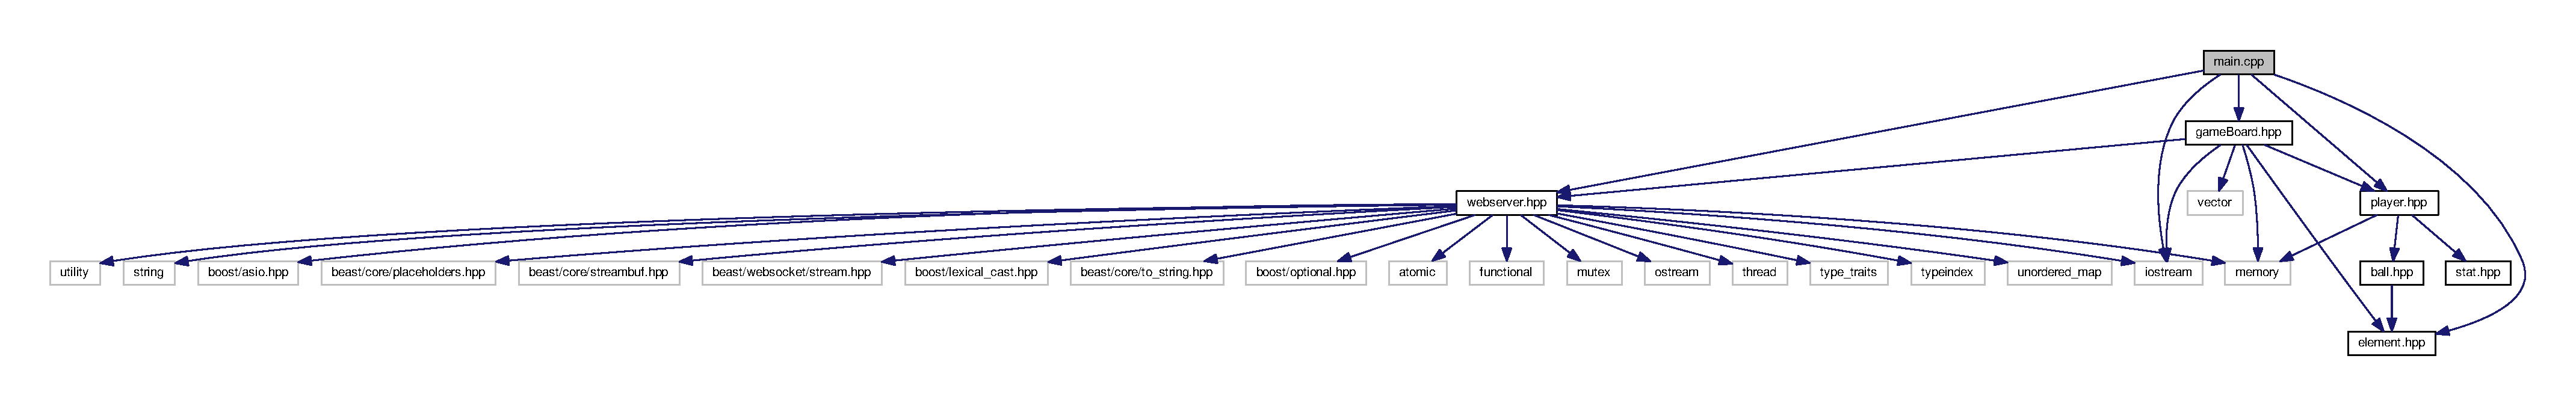
\includegraphics[width=350pt]{main_8cpp__incl}
\end{center}
\end{figure}
\subsection*{Functions}
\begin{DoxyCompactItemize}
\item 
int {\bfseries main} (int argc, char $\ast$argv\mbox{[}$\,$\mbox{]})\hypertarget{main_8cpp_a0ddf1224851353fc92bfbff6f499fa97}{}\label{main_8cpp_a0ddf1224851353fc92bfbff6f499fa97}

\end{DoxyCompactItemize}


\subsection{Detailed Description}
\begin{DoxyAuthor}{Author}

\end{DoxyAuthor}
\begin{DoxyDate}{Date}

\end{DoxyDate}

%--- End generated contents ---

% Index
\backmatter
\newpage
\phantomsection
\clearemptydoublepage
\addcontentsline{toc}{chapter}{Index}
\printindex

\end{document}
